In the previous section, we showed that there are a number of margins on which clustering methodologies are sensitive:  uncertainty in the input data and the choice of the number of clusters. However, these issues are only important for empirical labor economists to the extent that these
sensitivities impact empirical estimates in a meaningful way. To that end, in this section, we demonstrate the impact these issues have on the empirical findings of a well-known paper that uses commuting zones.

\citet{ADH2013} (hereafter, ADH) estimate the impact that increased trade competition from China had on manufacturing employment in the United States. The magnitude of the main finding has been widely discussed and debated in economics and in the popular press.\footnote{For example, see The Economist, March 11, 2017 ``Economists argue about the impact of Chinese imports on America'' \url{http://www.economist.com/news/finance-and-economics/ 21718513-china-shock-has-not-been-debunked-it-worth-understanding}.} To estimate this effect empirically, they use variation in the initial distribution of manufacturing employment at the commuting zone level, and national increases in imports from China by manufacturing subsector. Because ADH use commuting zones as their definition of local labor markets, their empirical analysis may be impacted by the issues outlined above.\footnote{We want to acknowledge that the authors have been incredibly helpful in the process of replicating their paper, both in providing data and helping to troubleshoot, and were receptive to this exercise.}

Their main estimating equation in the paper is as follows:

\begin{equation}\label{eqn:adh}
\Delta L_{it}^m = \gamma_t + \beta_1 \Delta IPW_{uit} + \beta_2 X_{it} + e_{it}
\end{equation}

Where $\Delta L_{it}^m$ is the decadal change in manufacturing employment in Commuting Zone $i$ following year $t$, $\Delta IPW_{uit}$ is the import exposure measure for the United States, and $X_{it}$ are control variables. All regressions are weighted by population share of the commuting zone.

\subsection{Replication of ADH}
\FloatBarrier
Since we use slightly different methods of aggregating data, we compare the main estimates from ADH (Table 1 in their paper) to our replication, which we show in Table \ref{tab:adhreplication}.\footnote{ADH use individual level IPUMS data, which as a PUMA geography, and assign those observations to commuting zones based on population weights (more detail at \url{http://www.ddorn.net/data.htm}). We just use county-level tabulations, which aggregate to the commuting zone level.} Each cell in the table is a coefficient from a different regression, and for simplicity we just display estimates for the time period 1990-2000 (other results available upon request). The first column shows the estimates from their paper, while the second column changes the import exposure measures to our replicated measure. In the third column, we use our estimate of the change in manufacturing employment and weights. The final column clusters on commuting zone rather than state.

% source: name of SAS program
% Last updated:

\begin{table}\centering
\caption{China Syndrome Replication and Comparison, 1990-2000 \label{tab:adhreplication}}
\begin{tabular}{lcccc}
\hline\hline
       & ADH Estimate & Our RHS & Our LHS and Weight & CZ Clustering  \\
       \hline
$\Delta IPW_{cz,t}$ & -0.8875 & -0.8871 & -0.8748 & -0.8748 \\
                   & (0.1812) & (0.1811) & (0.1527) & (0.1243) \\

\hline
\multicolumn{5}{p{6in}}{\footnotesize \textit{Notes}: Table from author's calculations, using data from \citet{ADH2013} and constructed data, based on equation \ref{eqn:adh}. Column 1 is Table 2, Column 1 from ADH (2013). Column 2 replaces their measure of import exposure to ours. Column 3 replaces their measure of change in manufacturing employment and CZ-specific weights with ours. Column 4 does not cluster on state. Standard errors are in parentheses. All coefficients are significant with p-values less than 0.01.}\\
\end{tabular}
\end{table}



Overall, the estimates are considerably stable, giving us confidence that we are properly replicating their main finding. We now turn to demonstrating how these estimates are affected by the concerns with the commuting zone definitions themselves.

\subsection{Sensitivity to Errors in Flows Data}

To demonstrate how sensitive the results of Equation \ref{eqn:adh} are to different commuting definitions, we re-estimate the equation using the 1000 realizations of commuting zones that were generated in the previous section.

\begin{figure}\centering
\caption{Distribution of Effect, 1990-2000 \label{fig:1990dist}}
\begin{tabular}{c}
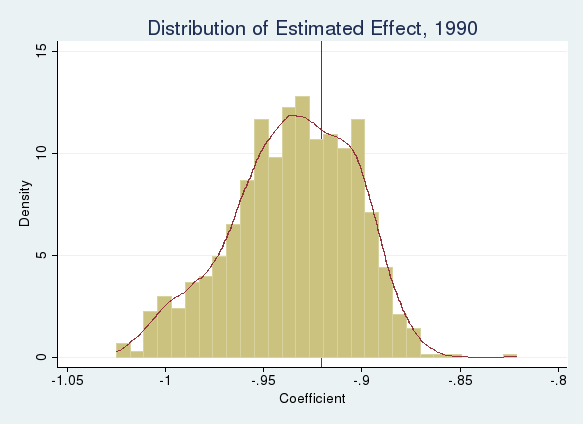
\includegraphics[scale=.5]{./figures/1990_distribution.png}\\
\multicolumn{1}{p{4.5in}}{\footnotesize \emph{Note:} Histogram plots estimates of $\beta_1$ from equation \ref{eqn:adh}, based on commuting zone realizations as outlined in Section \ref{sec:dsens}.}
\end{tabular}
\end{figure}

 The coefficients from this exercise are graphed in Figure \ref{fig:1990dist}, which shows the distribution of the estimated effect for the 1990-2000 period. The red vertical line shows the estimate using the published flows data from our national replication of TS1990. However, this value is actually more negative than about 75\% of the rest of the values, and there is a long negative tail. However, the values are within two standard errors of the original estimate.

Another way to summarize the results of this exercise is to look at the distribution of t-statistics, which incorporates information about $se_{\beta_1}$ into the analysis as well, and comparing that distribution to the critical values. To use the distribution of t-statistics in an empirical setting, researchers construct a 95\% confidence interval of the t-statistic by using the values at the 97.5th and 2.5th percentiles of the 1000 realizations. If this confidence interval is outside the critical value $t_{0.025}$, then the null hypothesis can be rejected at $\alpha = 0.05$. 

To give an empirical application, Figure \ref{fig:1990_tdist} shows the distribution of t-statistics obtained from estimating \ref{eqn:adh}. The blue vertical line is the original t-statistic, and the light gray vertical lines are the 2.5th and 97.5th percentiles. Clearly, in this application the result is still significant, because the entire confidence interval of t-statistics is less than the critical value ($-1.96$).

\begin{figure}\centering
\caption{Distribution of T-Statistic, 1990-2000 \label{fig:1990_tdist}}
\begin{tabular}{c}
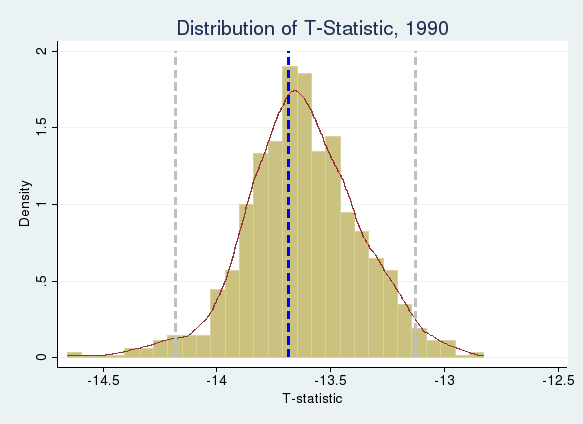
\includegraphics[scale=.5]{./figures/1990_tstat_distribution.png}\\
\multicolumn{1}{p{4.5in}}{\footnotesize \emph{Note:} Histogram plots t-statistics derived from estimating  equation \ref{eqn:adh}, based on commuting zone realizations as outlined in Section \ref{sec:dsens}.}
\end{tabular}
\end{figure}

This exercise demonstrates that there is additional uncertainty induced by the construction of the commuting zones that is not addressed in empirical estimates that use these definitions, which may overstate the precision of the results.

\subsection{Sensitivity to Chosen Cutoff}

In addition to the uncertainty that is induced by underlying errors in the commuting flows, in Section 3.2 we showed that the decision of where to stop the clustering process was rather arbitrary, since there is no clear guidance on what cutoff is most appropriate. To demonstrate how the cutoff choice affects estimates of $\beta_1$ from Equation \ref{eqn:adh}, we generate clusters based on cutoffs between 0.9 and 0.97 and estimate the equation using the resulting clusters.

\begin{figure}\centering
\caption{Differences in Effect Based on Cluster Cutoff \label{fig:cutoff_dist}}
\begin{tabular}{cc}

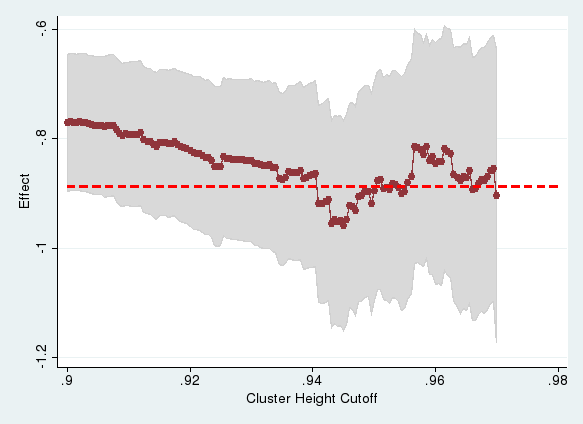
\includegraphics[scale=.35]{./figures/cutoff_1990_1.png} & 
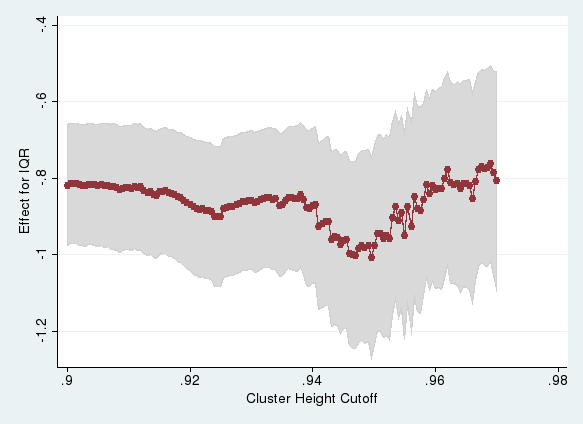
\includegraphics[scale=.35]{./figures/cutoff_iqr_1990_1.png}\\
(a) Effect by Cutoff Height & (b) Effect by Cutoff Height, Scaled by IQR \\
\multicolumn{2}{p{6.5in}}{\footnotesize \emph{Note:} Author's calculations based on replication of Tolbert and Sizer's method. Panel (a) shows estimates of $\beta_1$ from equation \ref{eqn:adh} for different definitions of commuting zones based on height cutoff, while Panel (b) shows estimates of $\beta_1$ scaled by the difference in exposure between the 25th and 75th percentile commuting zone. The horizontal line in panel (a) is the main estimate from \citet{ADH2013}}
\end{tabular}
\end{figure}

Figure \ref{fig:cutoff_dist} displays the results of this exercise, where panel (a) shows the raw coefficient and panel (b) shows the coefficient scaled by the interquartile range of $\Delta IPW_{uit}$, since the IQR changes based on the composition of the clusters. In panel (a),  the red horizontal line is the estimate from ADH.

Again, our results show that there is some variation in the estimate based on the cutoff value. Around the cutoff value that most closely replicates TS1990 ($0.9418$), the estimate is the most negative. However, cutoff values marginally higher or lower give different results, because the number of clusters changes quickly at that point. Given the sensitivity of estimates to the chosen cutoff, best practices for a researcher would be to report estimates for a broad range of possible cutoffs.	

\subsection{Advice to Researchers}

From the results above, it is clear that current commuting zone definitions understate the uncertainty of zone assignment, which has implications for empirical results. Importantly, this uncertainty manifests itself on two different margins: uncertainty about zone assignment due to errors in the flows, and uncertainty about zone assignment due to the chosen cutoff. 

Given this uncertainty, we have two pieces of advice for researchers using commuting zones. First, we suggest re-estimating results using all realizations of commuting zones, which incorporates the additional uncertainty because of the underlying error in the flows. Researchers can do this either by using the distribution of $\beta$ or the distribution of the t-statistics, as described in the previous sub-sections. Second, we suggest displaying results for a variety of different cutoff values. This second point is particularly important for researchers applying the  methodology from TS to data outside the United States, given that results can differ considerably. 

To aid researchers in this effort, we provide datasets and code online that include a crosswalk from county to all the realizations of commuting zones, as well as commuting zones for different cutoff values.\footnote{Our code is available at \url{https://github.com/larsvilhuber/MobZ/}, see also \citet{mobzrepl201704}.} We also provide our sample code that produced Figures \ref{fig:1990dist} and \ref{fig:cutoff_dist}.



